\documentclass[10pt,letterpaper]{article}
\usepackage{multicol}
\usepackage{calc}
\usepackage{ifthen}
\usepackage[landscape]{geometry}
\usepackage{hyperref}
\usepackage{amsmath}
\usepackage{graphicx}

% To make this come out properly in landscape mode, do one of the following
% 1.
%  pdflatex latexsheet.tex
%
% 2.
%  latex latexsheet.tex
%  dvips -P pdf  -t landscape latexsheet.dvi
%  ps2pdf latexsheet.ps


% If you're reading this, be prepared for confusion.  Making this was
% a learning experience for me, and it shows.  Much of the placement
% was hacked in; if you make it better, let me know...


% 2008-04
% Changed page margin code to use the geometry package. Also added code for
% conditional page margins, depending on paper size. Thanks to Uwe Ziegenhagen
% for the suggestions.

% 2006-08
% Made changes based on suggestions from Gene Cooperman. <gene at ccs.neu.edu>


% To Do:
% \listoffigures \listoftables
% \setcounter{secnumdepth}{0}


% This sets page margins to .5 inch if using letter paper, and to 1cm
% if using A4 paper. (This probably isn't strictly necessary.)
% If using another size paper, use default 1cm margins.
\ifthenelse{\lengthtest { \paperwidth = 11in}}
	{ \geometry{top=.5in,left=.5in,right=.5in,bottom=.5in} }
	{\ifthenelse{ \lengthtest{ \paperwidth = 297mm}}
		{\geometry{top=1cm,left=1cm,right=1cm,bottom=1cm} }
		{\geometry{top=1cm,left=1cm,right=1cm,bottom=1cm} }
	}

% Turn off header and footer
\pagestyle{empty}
 

% Redefine section commands to use less space
\makeatletter
\renewcommand{\section}{\@startsection{section}{1}{0mm}%
                                {-1ex plus -.5ex minus -.2ex}%
                                {0.5ex plus .2ex}%x
                                {\normalfont\large\bfseries}}
\renewcommand{\subsection}{\@startsection{subsection}{2}{0mm}%
                                {-1explus -.5ex minus -.2ex}%
                                {0.5ex plus .2ex}%
                                {\normalfont\normalsize\bfseries}}
\renewcommand{\subsubsection}{\@startsection{subsubsection}{3}{0mm}%
                                {-1ex plus -.5ex minus -.2ex}%
                                {1ex plus .2ex}%
                                {\normalfont\small\bfseries}}
\makeatother

% Define BibTeX command
\def\BibTeX{{\rm B\kern-.05em{\sc i\kern-.025em b}\kern-.08em
    T\kern-.1667em\lower.7ex\hbox{E}\kern-.125emX}}

% Don't print section numbers
\setcounter{secnumdepth}{0}


\setlength{\parindent}{0pt}
\setlength{\parskip}{0pt plus 0.5ex}

\DeclareMathOperator*{\argmin}{arg\,min}
\DeclareMathOperator*{\argmax}{arg\,max}


% -----------------------------------------------------------------------

\begin{document}

\raggedright
\footnotesize
\begin{multicols}{3}


% multicol parameters
% These lengths are set only within the two main columns
%\setlength{\columnseprule}{0.25pt}
\setlength{\premulticols}{1pt}
\setlength{\postmulticols}{1pt}
\setlength{\multicolsep}{1pt}
\setlength{\columnsep}{2pt}

\begin{center}
     \Large{\textbf{Machine Learning Cheat Sheet}} \\
\end{center}

\section{Estimating Parameters}

\subsection{Likelihood of $\theta$ given the sample D}

\begin{equation*}
l(\theta | D) = p(D | \theta) = \prod_t p(x^t | \theta)
\end{equation*}

\subsection{Log likelihood}
\begin{equation*}
L(\theta | D) = \log l(\theta | D) = \sum_t \log p(x^t | \theta)
\end{equation*}

\subsection{Maximum Likelihood Estimation (MLE)}

\begin{equation*}
	\theta_{MLE} = \underset{\theta}{\argmax} \ L(\theta | D)
\end{equation*}

\subsection{Bernoulli}
\begin{equation*}
P(x) = p_0^x(1-p_0)^{(1-x)}
\end{equation*}
\begin{equation*}
L(p_0 | D) = \log \prod_t p_0^{x^t}(1-p_0)^{(1-x^t)}
\end{equation*}
\begin{equation*}
MLE: p_0 = \sum_t x^t / N
\end{equation*}
\begin{align*}
\theta_{MLE} &= \argmax_{\theta} L(p_0 | D) \\ 
&= \argmax_{\theta} \log \prod_t p_0^{x^t}(1-p_0)^{(1-x^t)} \\
&= \argmax_{\theta} \sum_t \log p_0^{x^t}(1-p_0)^{(1-x^t)} \\
&= \argmax_{\theta} \sum_t [x^t \log p_0 + (1 - x^t) \log(1 - p_0)]
\end{align*}
\begin{align*}
\frac{\partial L(p_0|D)}{\partial p_0} &= 0 \\
\frac{\partial L(p_0|D)}{\partial p_0} &=
\frac{\sum_t x^t}{p_0} + \frac{\sum_t (1 - x^t)}{(1 - p_0)} = 0 \\
(\sum_{i=1}^{n} x_i) \cdot (1 - \theta) &= \theta \cdot \sum_{i=1}^{n} (1-x_i) \\ 
\sum_{t} x^t - \theta \cdot \sum_{t} &= \theta \cdot \sum_{t} (1-x^t) \\ 
\theta = \frac{\sum_{t} x^t}{\sum_{t} x^t + \sum_{t} (1-x^t)} &= \frac{n_1}{n}
\end{align*}

\subsection{Gaussian (Normal)}

\begin{align*}
p(\theta) &= \frac{1}{\sqrt{2 \pi} \sigma_1} e ^{-\frac{(\theta - \mu_1)^2}{2 \sigma_1^2}} \\
p(x | \theta) &= \frac{1}{\sqrt{2 \pi} \sigma_2} e ^{-\frac{(x - \theta)^2}{2 \sigma_2^2}} \\
\theta_{MLE} &= \argmax_{\theta} p(\theta | D ) = \argmax_{\theta} p(D |\theta) p(\theta) \\
&= \argmax_{\theta} \log(p(D |\theta) p(\theta)) \\
&= \argmax_{\theta} \log p(D |\theta) + \log p(\theta) \\
\end{align*}
\begin{align*}
&= \argmax (- \frac{1}{2} \log 2 \pi \sigma_2^2 - \frac{(x-\theta)^2}{2\sigma_2^2} - \frac{1}{2}\log 2 \pi \sigma_1^2 - \frac{(\theta - \mu_1)^2}{2 \sigma_1^2} ) \\
&= \argmax (-\frac{(x-\theta)^2}{2\sigma_2^2} - \frac{(\theta - \mu_1)^2}{2 \sigma_1^2})
\end{align*}
$\frac{\partial}{\partial \theta} (-\frac{(x-\theta)^2}{2\sigma_2^2} - \frac{(\theta - \mu_1)^2}{2 \sigma_1^2}) = 0$ \\
$\frac{x-\theta}{\sigma_2^2} - \frac{\theta - \mu_1}{ \sigma_1^2} = \sigma_1^2 (x-\theta) - \sigma_2^2(\theta - \mu_1) = 0$\\
$\theta = \frac{\sigma_1^2}{\sigma_1^2 + \sigma_2^2} x + \frac{\sigma_2^2}{\sigma_1^2 + \sigma_2^2} \mu_1$  

\subsection{Maximum a Posteriori (MAP)}

\begin{align*}
	\underset{\theta}{\argmax} \ P(\theta | D) &= \underset{\theta}{\argmax} \ \frac{P(D | \theta) P(\theta)}{P(D)} \\
	&= \underset{\theta}{\argmax} \ P(D | \theta) P(\theta)
\end{align*}

\section{Linear discriminant analysis}

\subsection{Two Classes}

\begin{align*}
g(x) &= g_1(x) - g_2(x) = (w_1^T x +w_{10}) - (w_2^T x +w_{20}) \\
&= (w_1 - w_2)^T x + (w_{10} - w_{20}) = w^T x + w_0
\end{align*}\\

$choose \begin{cases}
C_1 \quad \text{if }g(x) > 0 \\
C_2 \quad \text{otherwise}
\end{cases}$

\subsection{Logistic discrimination}

$\log \frac{p(x|C_1)}{p(x|C_2)} = w^Tx + w_0$

\section{Regression}

\subsection{Linear regression}

Find optimal $w$ and $w_0$ such that the average distance of points from the line is minimized.

\begin{equation*}
\underset{w,w_0}{\argmax} \ \sum_{t} \frac{1}{2} \left( w x^t + w_0 - r^t \right)^2
\end{equation*}

Differentiate, and solution is

\begin{equation*}
\left[ \sum_{t} x^t (x^t)^T \right] w = \sum_{t} r^t x^t
\end{equation*}

\subsection{In one dimension}
\begin{equation*}
g(x^t, w_1,w_0) = w_1 x^t + w_0	
\end{equation*}

$\begin{cases}
\sum_t r^t &= N w_0 +w_1 \sum_t x^t	\\
\sum_t r^t x^t &= w_0 \sum_t x^t +w_1 \sum_t (x^t)^2	
\end{cases}$

$A =\begin{bmatrix}
    N & \sum_t x^t \\
    \sum_t x^t & \sum_t (x^t)^2 \\
\end{bmatrix}$ \quad
$w = \begin{bmatrix} w_0 \\ w_1\end{bmatrix}$ \quad
$y = \begin{bmatrix} \sum_t r^t \\ \sum_t r^t x^t\end{bmatrix}$
\begin{equation*}
w = A^-1 y	
\end{equation*}

\subsection{Polynomial linear regression}

$D =\begin{bmatrix}
    1 & x_{1}^{1} & x_{2}^{1} & \dots & x_{k}^{1} \\
    1 & x_{1}^{2} & x_{2}^{2} & \dots & x_{k}^{2} \\
    \dots & \dots & \dots &\dots & \dots \\
    1 & x_{1}^{N} & x_{2}^{N} & \dots & x_{k}^{N} \\
\end{bmatrix}$ \qquad
$r = 
\begin{bmatrix}
r^1 \\
r^2 \\
\dots \\
r^N     
\end{bmatrix}
$ \\
\text{ }\\

$w = (D^T D)^{-1} D^T r$

\begin{equation*}
g(x) = w_k x_k + w_{k−1} x_{k−1} + \cdots + w_1 x_1 + w_0
\end{equation*}

\subsection{Error measures}
Squared error:\\
\begin{equation*}
Err(g, D) = \frac{1}{2} \sum_k [r^k - g(x^t)]^2 	
\end{equation*}

Mean squared error:\\
\begin{equation*}
Err(g, D) = \frac{1}{N} \sum_k [r^k - g(x^t)]^2 	
\end{equation*}

Absolute error:\\
\begin{equation*}
Err(g, D) = \sum_k [r^k - g(x^t)]
\end{equation*}
\subsection{Regularization}

Regularization is the technique of adding an additional term to an error function (which measures prediction error) called a penalty term, that is higher if a hypothesis is more complex in some way. It is used to try to avoid overfitting.

\section{Classification}

\subsection{Bayes' rule}
\begin{equation*}
P(C_i|D) = \frac{P(C_i) p(D|C_i)}{p(D)}
\rightarrow posterior = \frac{prior \cdot likelihood}{evidence}
\end{equation*}

$\sum_i P(C_i) = 1$\\
$p(D) = \sum_i P(C_i)p(D|C_i)$\\
$\sum_i p(C_i | D) = 1$\\

For $prior = p(\theta)$ \\
$p(D) = \int_{\theta} P(\theta) p(D|\theta)$

\subsection{Naive Bayes}
Assumes that features are independent.\\
\emph{Classifies} input vector $D = <x_1, ..., x_k>$ as class $C_i$ according to
\begin{align*}
	\underset{i}{\argmax} \ P(C_i | D)
	&= \underset{i}{\argmax} \ P(x_1, ..., x_n | C_i) P(C_i)\\
	&= \underset{i}{\argmax} \ P(C_i) \prod_{k}^{n} P(x_k | C_i)
\end{align*}

\begin{itemize}
	\item \emph{Discrete $x_k$} -- $P(x_k | C_i) = \frac{count(X_k = x_k, C_i)}{count(C_i)}$
	
	For smoothing $m$, use $P(x_k | C_i) = \frac{count(X_k = x_k, C_i) + m}{count(C_i) + N \cdot m}$, where $N$ is the number of different possible values for $X_k$
	\item \emph{Continuous $x_k$} -- Can use any PDF, but usually use Gaussian $P(x_k | C_i) = \mathcal{N}(\mu, \sigma^2) = \frac{1}{\sqrt{2 \pi}\sigma} e^{-\frac{(x_k-\mu)^2}{2\sigma^2}} $, where $\mu$ and $\sigma$ are, respectively, the average and variance. The Gaussian distribution already provides smoothing.
\end{itemize}

\subsection{Losses and Risks}

\begin{tabular}{ | l | l l l | } 
\hline
& \multicolumn{3}{|c|}{Class} \\
Action & $C_1$ & $\cdots$ & $C_k$  \\
\hline
$\alpha_1$ & $\lambda_{11}$ & $\cdots$ &  $\lambda_{1k}$  \\
$\cdots$ & $\cdots$ & $\cdots$ & $\cdots$\\
$\alpha_i$ & $\lambda_{i1}$ & $\cdots$ & $\lambda_{ik}$  \\
\hline
\end{tabular}

\begin{equation*}
R(\alpha_i | D) = \sum_k \lambda_{ik} P(C_k | D)
\end{equation*}
Choose $\alpha_i$ if $R(\alpha_i | D) = \argmin_k R(\alpha_k|D)$\\

\section{Bias-Variance decomposition}

\begin{equation*}
mse(\hat \theta) = bias(\hat \theta)^2  + variance(\hat \theta)
\end{equation*}
$\mu = E[\hat \theta]$
\begin{align*}
mse(d) &= E[(\hat \theta - \theta)^2] = E[((\hat \theta - \mu) + (\mu - \theta))^2] \\
&= E[(\hat \theta - \mu)^2 +2(\hat \theta - \mu)(\mu - \theta)+ (\mu - \theta)^2] \\
&=E[(\hat \theta - \mu)^2] + E[(\mu - \theta)^2] \\
&= variance(\hat \theta) + bias(\hat \theta)^2 
\end{align*}

\subsection{Bias-–variance tradeoff}
\begin{itemize}
	\item The bias is an error from erroneous assumptions in the learning algorithm. High bias can cause an algorithm to miss the relevant relations between features and target outputs (underfitting).
	\item The variance is an error from sensitivity to small fluctuations in the training set. High variance can cause an algorithm to model the random noise in the training data, rather than the intended outputs (overfitting).
\end{itemize}

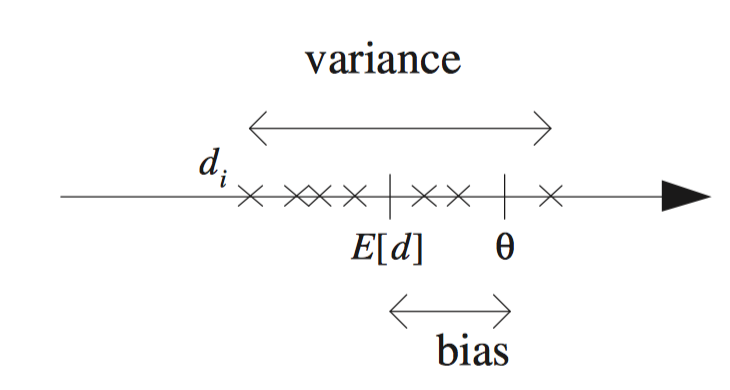
\includegraphics[scale=.6]{images/bias-variance.png}

$\theta$ is the parameter to be estimated. $d_ii$ are several estimates (denoted by '×') over different samples $X_i$ . Bias is the difference between the expected value of $d$ and $\theta$. Variance is how much $d_i$ are scattered around the expected value. We would like both to be small.

\section{Bias of an estimator}
Let $d = d(X)$ be an estimator of $\theta$.

\begin{equation*}
bias_{\theta}(d) = E[d(X)] - \theta
\end{equation*}

If $bias_{\theta}(d)= 0$ for all $\theta$ values, then we say that $d$ is an unbiased estimator of $\theta$.

With $x^t$ drawn from some density with mean $\mu$, $E[\sum_t x^t] = N \mu$.

\section{Appendix}
\subsection{Transpose of a matrix}
Switch the row and column indices of the matrix.

$A =\begin{bmatrix}
    a_{1,1} & a_{1,2} & \dots & a_{1,j} \\
    a_{2,1} & a_{2,2} & \dots & a_{2,j} \\
    \dots & \dots & \dots  &\dots        \\
    a_{i,1} & a_{i,2} & \dots & a_{i,j} \\
\end{bmatrix}$  $A^T =\begin{bmatrix}
    a_{1,1} & a_{2,1} & \dots & a_{i,1} \\
    a_{1,2} & a_{2,2} & \dots & a_{i, 2} \\
    \dots & \dots & \dots  &\dots        \\
    a_{1,j} & a_{2, j} & \dots & a_{i, j} \\
\end{bmatrix}$

\subsection{Inverse of a matrix}
$\begin{bmatrix}
    a_{1,1} & a_{1,2} \\
    a_{2,1} & a_{2,2} \\
\end{bmatrix} ^{-1} = 
\frac{1}{a_{1,1} a_{2,2} - a_{1,2} a_{2,1}}
\begin{bmatrix}
	a_{2,2} & -a_{1,2} \\
    -a_{2,1} & a_{1,1} \\
\end{bmatrix}
$ \\
Generic matrix\\
$A = \begin{bmatrix}
    a_{1,1} & a_{1,2} & a_{1,3} \\
    a_{2,1} & a_{2,2} & a_{2,3} \\
    a_{3,1} & a_{3,2} & a_{3,3} \\
\end{bmatrix}$ \\ 

Calculate the "Matrix of Minors".\\
$A' = \begin{bmatrix}
    a_{1,1}' & a_{1,2}' & a_{1,3}' \\
    a_{2,1}' & a_{2,2}' & a_{2,3}' \\
    a_{3,1}' & a_{3,2}' & a_{3,3}' \\
\end{bmatrix}$\\

$a_{1,1}' = \begin{bmatrix}
    \bullet &  &  \\
    	 & a_{2,2} & a_{2,3} \\
    	 & a_{3,2} & a_{3,3} \\
\end{bmatrix} = a_{2,2} a_{3,3} - a_{2,3}a_{3,2}$

Apply a "checkerboard" of minuses to the "Matrix of Minors" and obtain the "Matrix of Cofactors". \\
$A' \rightarrow \begin{bmatrix}
    + & - & + \\
    - & + & - \\
    + & - & + \\
\end{bmatrix} \rightarrow A''$

Transpose the "Matrix of Cofactors"(Adjugate)

Multiply by 1/Determinant of the original matrix
$A^{-1} = \frac{1}{det(A)} (A'')^T$
\\
\smallskip
\rule{0.3\linewidth}{0.25pt}
\scriptsize

Copyright \copyright\ 2018 Antonio Mallia

\href{https://www.antoniomallia.it}{https://www.antoniomallia.it}

\end{multicols}
\end{document}
